\textbf{Anomaly detection \& Uncertainty.} The goal of this experiment is twofold: (1) it assesses the ability of the models to detect anomalies in asynchronous sequences, (2) it evaluates the quality of the predicted uncertainty on the categorical distribution. For this, we use a similar set-up as \citep{PriorNetworks}.

\textit{Set-up:} The experiments consist in introducing anomalies in datasets by changing the occurrence time of $10$\% of the events (at random after the time transformation described in appendix \ref{datasets}). Hence, the anomalies form out-of-distribution data, whereas unchanged events represent in-distribution data. The performance of the anomaly detection is assessed using Area Under Receiver Operating Characteristic (AUROC) and Area Under Precision-Recall (AUPR). We use two approaches: (i) We consider the \textit{categorical uncertainty} on $\bar{\bm{p}}(\DeltaTime)$, i.e., to detect anomalies we use the predicted probability of the true event as the anomaly score. (ii) We use the \textit{distribution uncertainty} at the observed occurrence time provided by our models. For \GPModel, we can evaluate  $q_\IndexClass(\DeltaTime)$ directly (difference of two normal distributions). For \DirModel, this probability does not have a closed-form solution so instead, we use the concentration parameters which are also indicators of out-of-distribution events. For all scores, i.e $\bar{\bm{p}}(\DeltaTime)_c$, $q_\IndexClass(\DeltaTime)$ and $\alpha_\IndexClass(\DeltaTime)$, a low value indicates a potential anomaly around time $\DeltaTime$.

\begin{figure}
\centering
    \begin{subfigure}{0.25\textwidth}
        \centering
        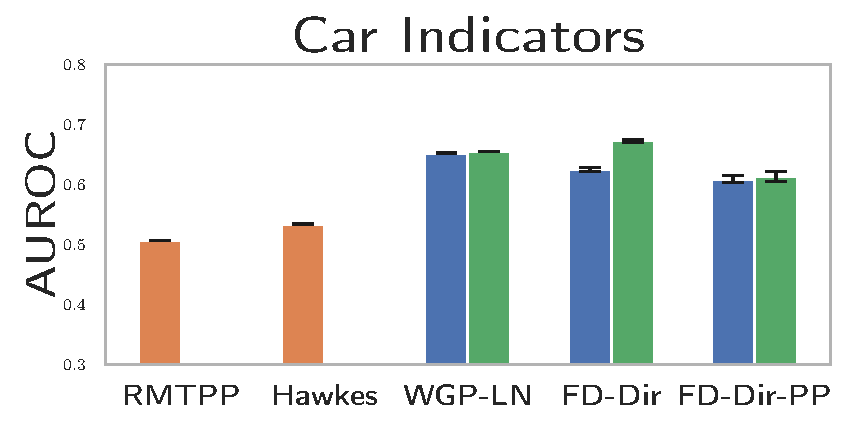
\includegraphics[width=\linewidth]{images/uncertainty-roc-bmw-indicator.pdf}
    \end{subfigure}%
    \begin{subfigure}{0.25\textwidth}
        \centering
        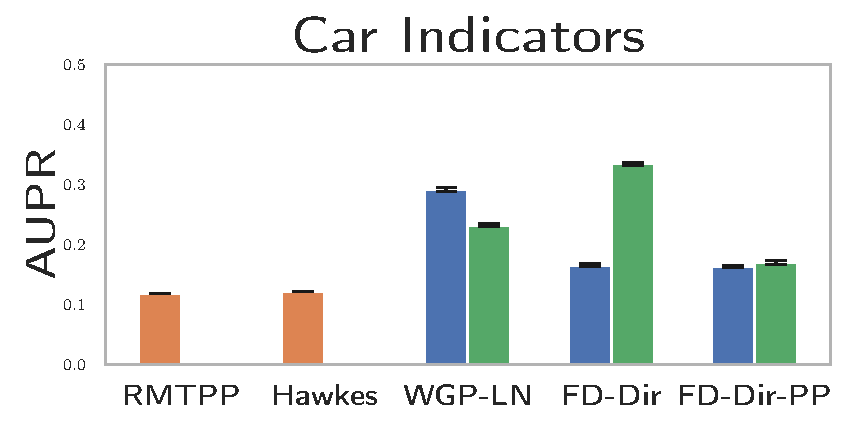
\includegraphics[width=\linewidth]{images/uncertainty-apr-bmw-indicator.pdf}
    \end{subfigure}%
        \begin{subfigure}{0.25\textwidth}
        \centering
        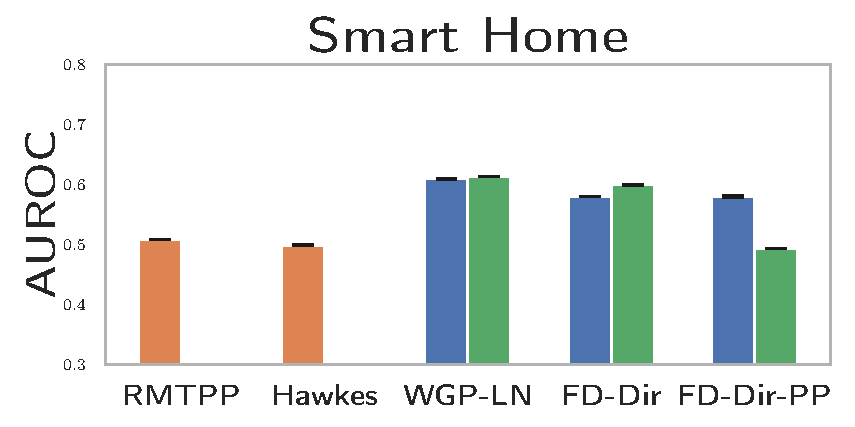
\includegraphics[width=\linewidth]{images/uncertainty-roc-kast-home.pdf}
    \end{subfigure}%
    \begin{subfigure}{0.25\textwidth}
        \centering
        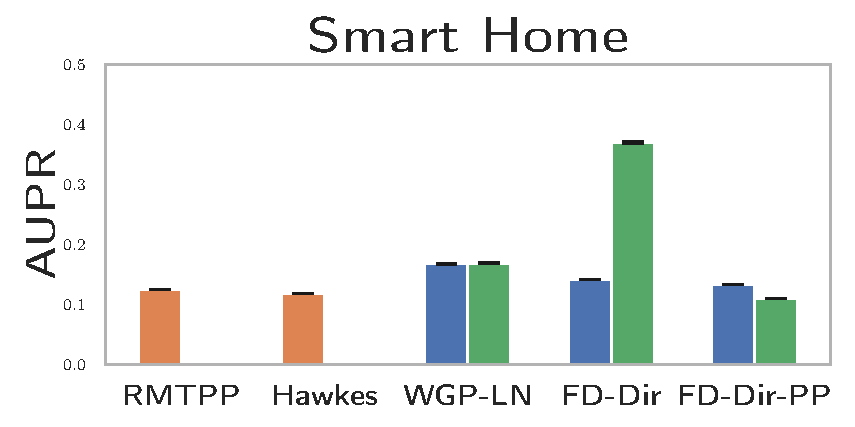
\includegraphics[width=\linewidth]{images/uncertainty-apr-kast-home.pdf}
    \end{subfigure}
    \caption{AUROC and APR comparison across dataset on anomaly detection. The orange and blue bars use categorical uncertainty score whereas the green bars use distributional uncertainty.}
    \label{fig:anomaly_detection}
    \vspace{-0.5cm}
\end{figure}

\textit{Results.} As seen in Fig.\ \ref{anomaly_detection}, the \DirModel and the \GPModel have particularly good performance. We observe that the \DirModel gives better results especially with distributional uncertainty. This might be due to the power of the concentration parameters that can be viewed as number of similar events around a given time.